\documentclass[12pt]{article}
\usepackage[top=1in, bottom=1.25in, left=1in, right=1in]{geometry}
\usepackage[]{graphicx}
\usepackage{amsmath}
\usepackage{multicol}
\usepackage{tikz}
\usepackage{authoraftertitle}
\usepackage{hyperref}
\setlength{\parindent}{0pt}
\setcounter{secnumdepth}{0}
\graphicspath{{images/}}

\tikzstyle{phase} = [rectangle, rounded corners, minimum width=3cm, minimum height=1cm, text centered, text width=3cm, draw=black]
\tikzstyle{arrow} = [thick, ->, >=stealth]

\title{
\begin{figure}[ht]
\centering
% \hspace{0.1cm}
% \begin{minipage}[b]{0.45\linewidth}

\includegraphics[scale=0.6]{Title_Photos.png}
% \end{minipage}
% \hspace{1cm}
% \begin{minipage}[b]{0.45\linewidth}
% 
\includegraphics[scale=0.45]{ETHenaLogo.png}
% \end{minipage}
\end{figure}\vspace{2cm}\\{\textbf{\Huge Luno Trading Challenge}} \vspace{1cm}\\ \textbf{{\Huge ETHena}}}
\date{}
\usepackage{authoraftertitle}
\author{\\
  \author{}Sanchit Ajmera\\
         \small{\affaddr{Department of Computing,}}\\
         \small{\affaddr{Imperial College London}} \\
         \small{\email{sanchitajmera2017@gmail.com}}
  \and \\
  \author{}Luqman Liaquat\\
         \small{\affaddr{Department of Computing,}}\\
         \small{\affaddr{Imperial College London}} \\
         \small{\email{luqman.liaquat90@gmail.com}}
  \and\\
  \author{}Manuj Mishra\\
         \small{\affaddr{Department of Computing,}}\\
         \small{\affaddr{Imperial College London}} \\
         \small{\email{manujmishra2000@gmail.com}}
  \and\\
  \author{}Shivam Patel\\
         \small{\affaddr{Department of Mathematics,}}\\
         \small{\affaddr{Imperial College London}} \\
         \small{\email{shivpatel1306@gmail.com}}
  \and\\
  \author{}Devam Savjani\\
         \small{\affaddr{Department of Computing,}}\\
         \small{\affaddr{Imperial College London}} \\
         \small{\email{devamsavjani@rocketmail.com}}
}
\begin{document}
\begin{titlepage}
    \maketitle
\end{titlepage}

\tableofcontents
\newpage
\begin{multicols}{2}
    \section{Motivation}

    We are a group of first year Imperial College London students, studying computing and mathematics. We all have an interest in trading and wanted to learn how we could implement algorithms to make useful and reliable predictions about the market. As a group of technically minded individuals, we were intrigued by blockchain and cryptocurrencies and this drew us to the Luno Challenge.
    \\
    Some of our team members have explored trading in the past and with our combined programming skills, we were confident that we could make a substantial profit. This competition has given us the opportunity to challenge ourselves and we have gained valuable insights into the world of blockchain, cryptocurrency and algorithmic trading.

    \section{Overview}
    \subsection{Luno API}
    Understanding and working with the Luno API was a vital step in producing a well-made bot. Our team chose to primarily implement our bot in Go despite having no experience in the language. This was because the Luno Go SDK had comprehensive documentation, allowing us to quickly and easily setup the foundations for our bots.
    \subsection{Historical Data}
    An important feature we built, using the Luno API $'GetTicker'$ function, was a live data collection and storage program on six currency pairs. As historical data was not natively available, we designed our own program to produce daily spreadsheet files with minute-interval data on bid and ask prices. We ensured this data collection was automated, backed up our data regularly, and included an anti-loss feature to prevent any possible errors from corrupting our file. The recent historical data we obtained was then used to carry out thorough backtesting on each iteration of our trading bots to measure progress and assess weaknesses. Once we were satisfied with the results, we deployed ETHena on the AWS server.

    \subsection{Performance Reports}
    We knew that iterative development, paired with constant performance reviews, was essential in fine-tuning ETHena. This led us to develop a utility feature which produced a daily report of ETHena's performance. The report featured an automatically generated graph which allowed us to pinpoint where a buy or sell order was executed and if it was the best decision in context of the market that day. An example of this graph can be found in the appendix (see Figure 1). Our performance report generation was a pivotal development and allowed us to identify several improvements that we would not have noticed otherwise.
    \subsection{Email Notifications}
    To deliver our performance reports in a convenient manner, we created an integrated email system. The system allowed us to receive notifications on important events that had occurred. These notifications covered trade histories, ETHena's status, and daily performance summaries which allowed each member to stay updated on ETHena's progress.
    \\
    Alongside the performance reports, the emails enabled us to carry out a more automated approach in development and execution.

    \section{Project flow}

    After our initial data collection, we started researching a host of trading strategies. We filtered through these and picked the most promising techniques (detailed below) which we then implemented and backtested. We did this multiple times on different data sets to allow us to fine-tune the variables without overfitting to a particular dataset. The final stage was to deploy the most successful bots onto the servers for live trading on the Luno market. As discussed, these bots underwent further testing and constant improvement throughout the competition.
    \begin{center}
        \scalebox{0.8}{
            \begin{tikzpicture}[node distance=1cm]
                \node (Research) [phase] {Research};
                \node (Development) [phase, bottom of=Research, yshift=-2cm] {Development};
                \node (Testing) [phase, bottom of=Development, yshift=-4cm] {Testing};
                \node (Deployment) [phase, bottom of=Testing, yshift=-6cm] {Deployment};

                \draw [arrow] (Research) -- (Development);
                \draw [arrow] (Development) -- (Testing);
                \draw [arrow] (Testing) -- (Deployment);
            \end{tikzpicture}}
    \end{center}
    \section{Research}
    An integral part of our project was to research strategic trading methods to predict market trends. Our team's intention was to go beyond this research by combining several strategies, indicators and risk management techniques to develop ETHena. Our core research has been summarised below.

    \subsection{Moving Average Convergence Divergence (MACD)}
    This was one of the first strategies we decided to explore and implement. The strategy considers two moving averages: long term and short term. New trends are identified when the two lines cross over. When a short term moving average crosses \textbf{above} a long term moving average it is known as a 'convergence' event signalling a new uptrend. The opposite (i.e. the short term average crossing \textbf{below} the long term average) is known as a divergence event, hence the name - Moving Average Convergence Divergence.

    \subsection{Relative Strength Index (RSI)}
    The Relative Strength Index is a momentum indicator, which is intended to chart the strength or weakness of a stock based on the closing prices of a recent trading period. It signals when an asset is overbought or oversold allowing one to make predictions on market trends. The RSI formula is:
    \begin{align*}
        RSI = & \ 100 -\frac{100}{1+RS}                           \\
        RS =  & \ \frac{\text{Average Gain}}{\text{Average Loss}}
    \end{align*}
    The \textbf{Average Gain} and \textbf{Average Loss} are calculated from the previous $n$ differences in close prices of each trading interval. For ETHena we used $n=14$ and varied the trading interval which allowed us to run bots with varying risk levels.
    \subsection{Exponential Moving Average (EMA)}
    Exponential Moving Average is a moving average which exponentially prioritises the more recent prices, whereas the simple moving average (SMA) equally prioritises all data points. Using the EMA over the SMA greatly improved the effectiveness of our MACD and RSI strategies.

    \subsection{Candlestick Analysis}
    After researching into strategies and speaking to day traders we found candlestick analysis to be one of the major indicators used when making decisions. This type of analysis involves spotting a variety of candlestick patterns including 123 Reversal, Hammer, Inverse Hammer, Three White Slaves and Morningstar, which can signal future trends.
    \subsection{EMA - Offset Algorithm}
    The Offset strategy buys when the price significantly drops and sells when the price significantly rises in comparison to the moving average. We used this strategy as we noticed there were multiple instances of the market suffering a huge loss and then recovering in a short time frame. This is also known colloquially as a Flash Crash.

    \subsection{Risk Management - Trailing Stoploss}
    The Trailing Stoploss strategy is used to determine when to sell by maximising profits and placing a fixed limit on potential losses. As the price rises the stoploss will rise with it. The value of the stoploss will always be proportional to the maximum price the asset has risen to since buying. Based on our backtesting, this stoploss ratio was set to 99.75\%. We also implemented an initial bail-out value such that an emergency sell order was triggered if an acquired asset significantly dropped in value immediately after buying. ETHena was set to bail after a 1\% immediate loss.\\\\
    \subsection{Final Choice}
    After backtesting on several different sets of data, we created ETHena, a bot which could trade using all of our strategies. We decided to use the Trailing Stoploss risk management feature by default to ensure our sell orders were placed at the best possible closing positions. This yielded substantial profit.
    \section{GUI}
    To help manage the bot, we created the ETHena GUI as shown below. The drop down menu for \textit{Name} allows us to choose who is running the bot, which then automatically selects their API keys. The sliders then allow us to set which strategies are being used and the weighting applied to each strategy. The time interval option sets how often calls to the market are made, effectively increasing or decreasing risk. The select option for \textit{Live} and \textit{Offline} allows one to decide whether to trade live or backtest on historical data. The final option then allows the user to select where the main.go file is stored on their system.\\\\
    
    
    \begin{minipage}[b]{1\linewidth}
        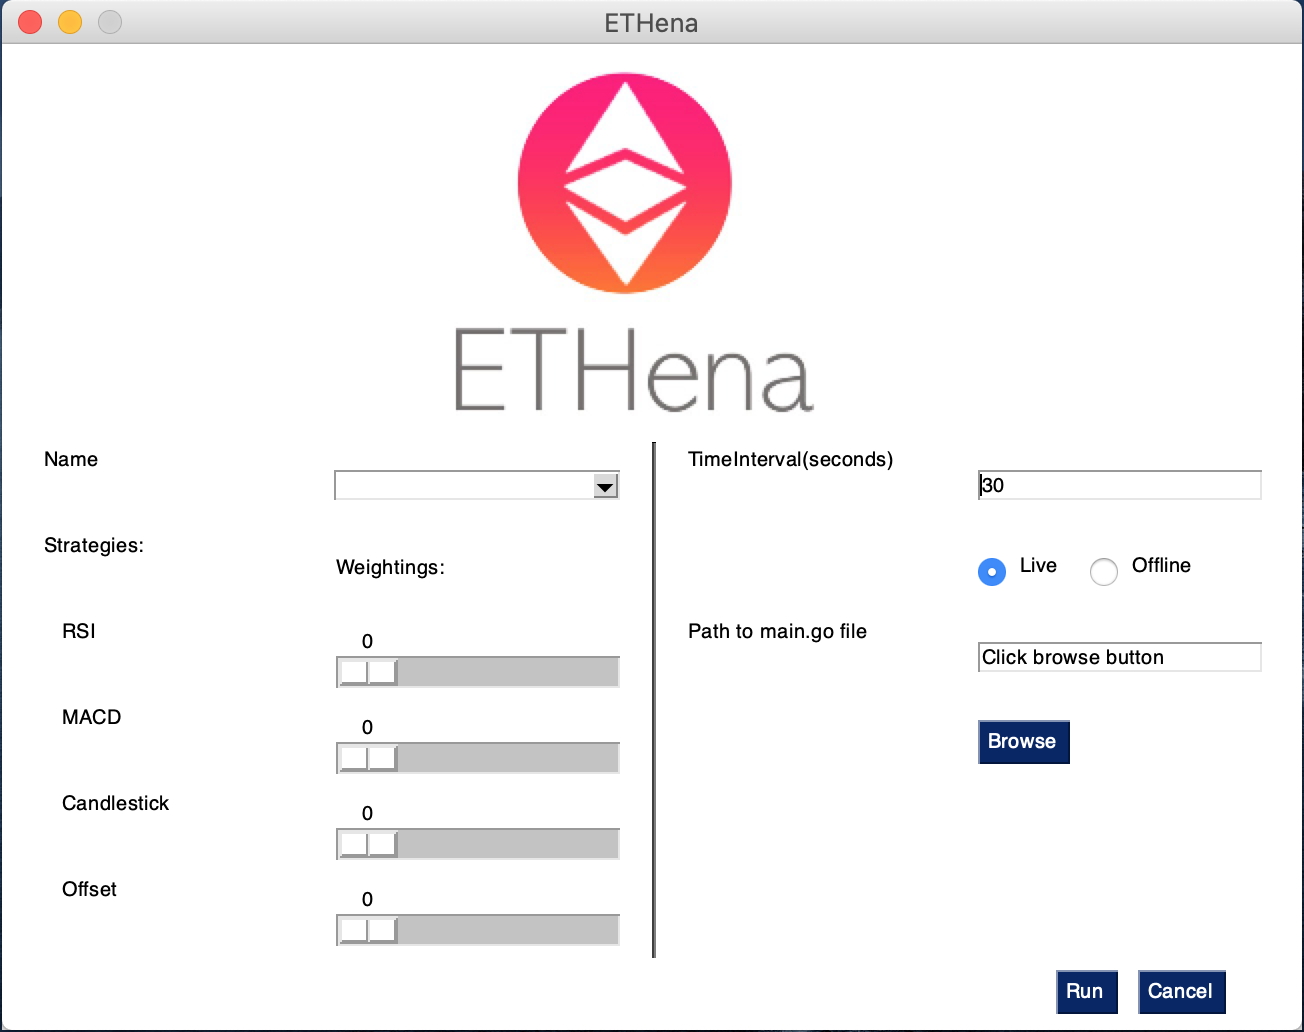
\includegraphics[width =\textwidth]{GUI-Image.png}
        \centering
        Figure 1: ETHena GUI
    \end{minipage}

    \begin{minipage}[b]{1\linewidth}
        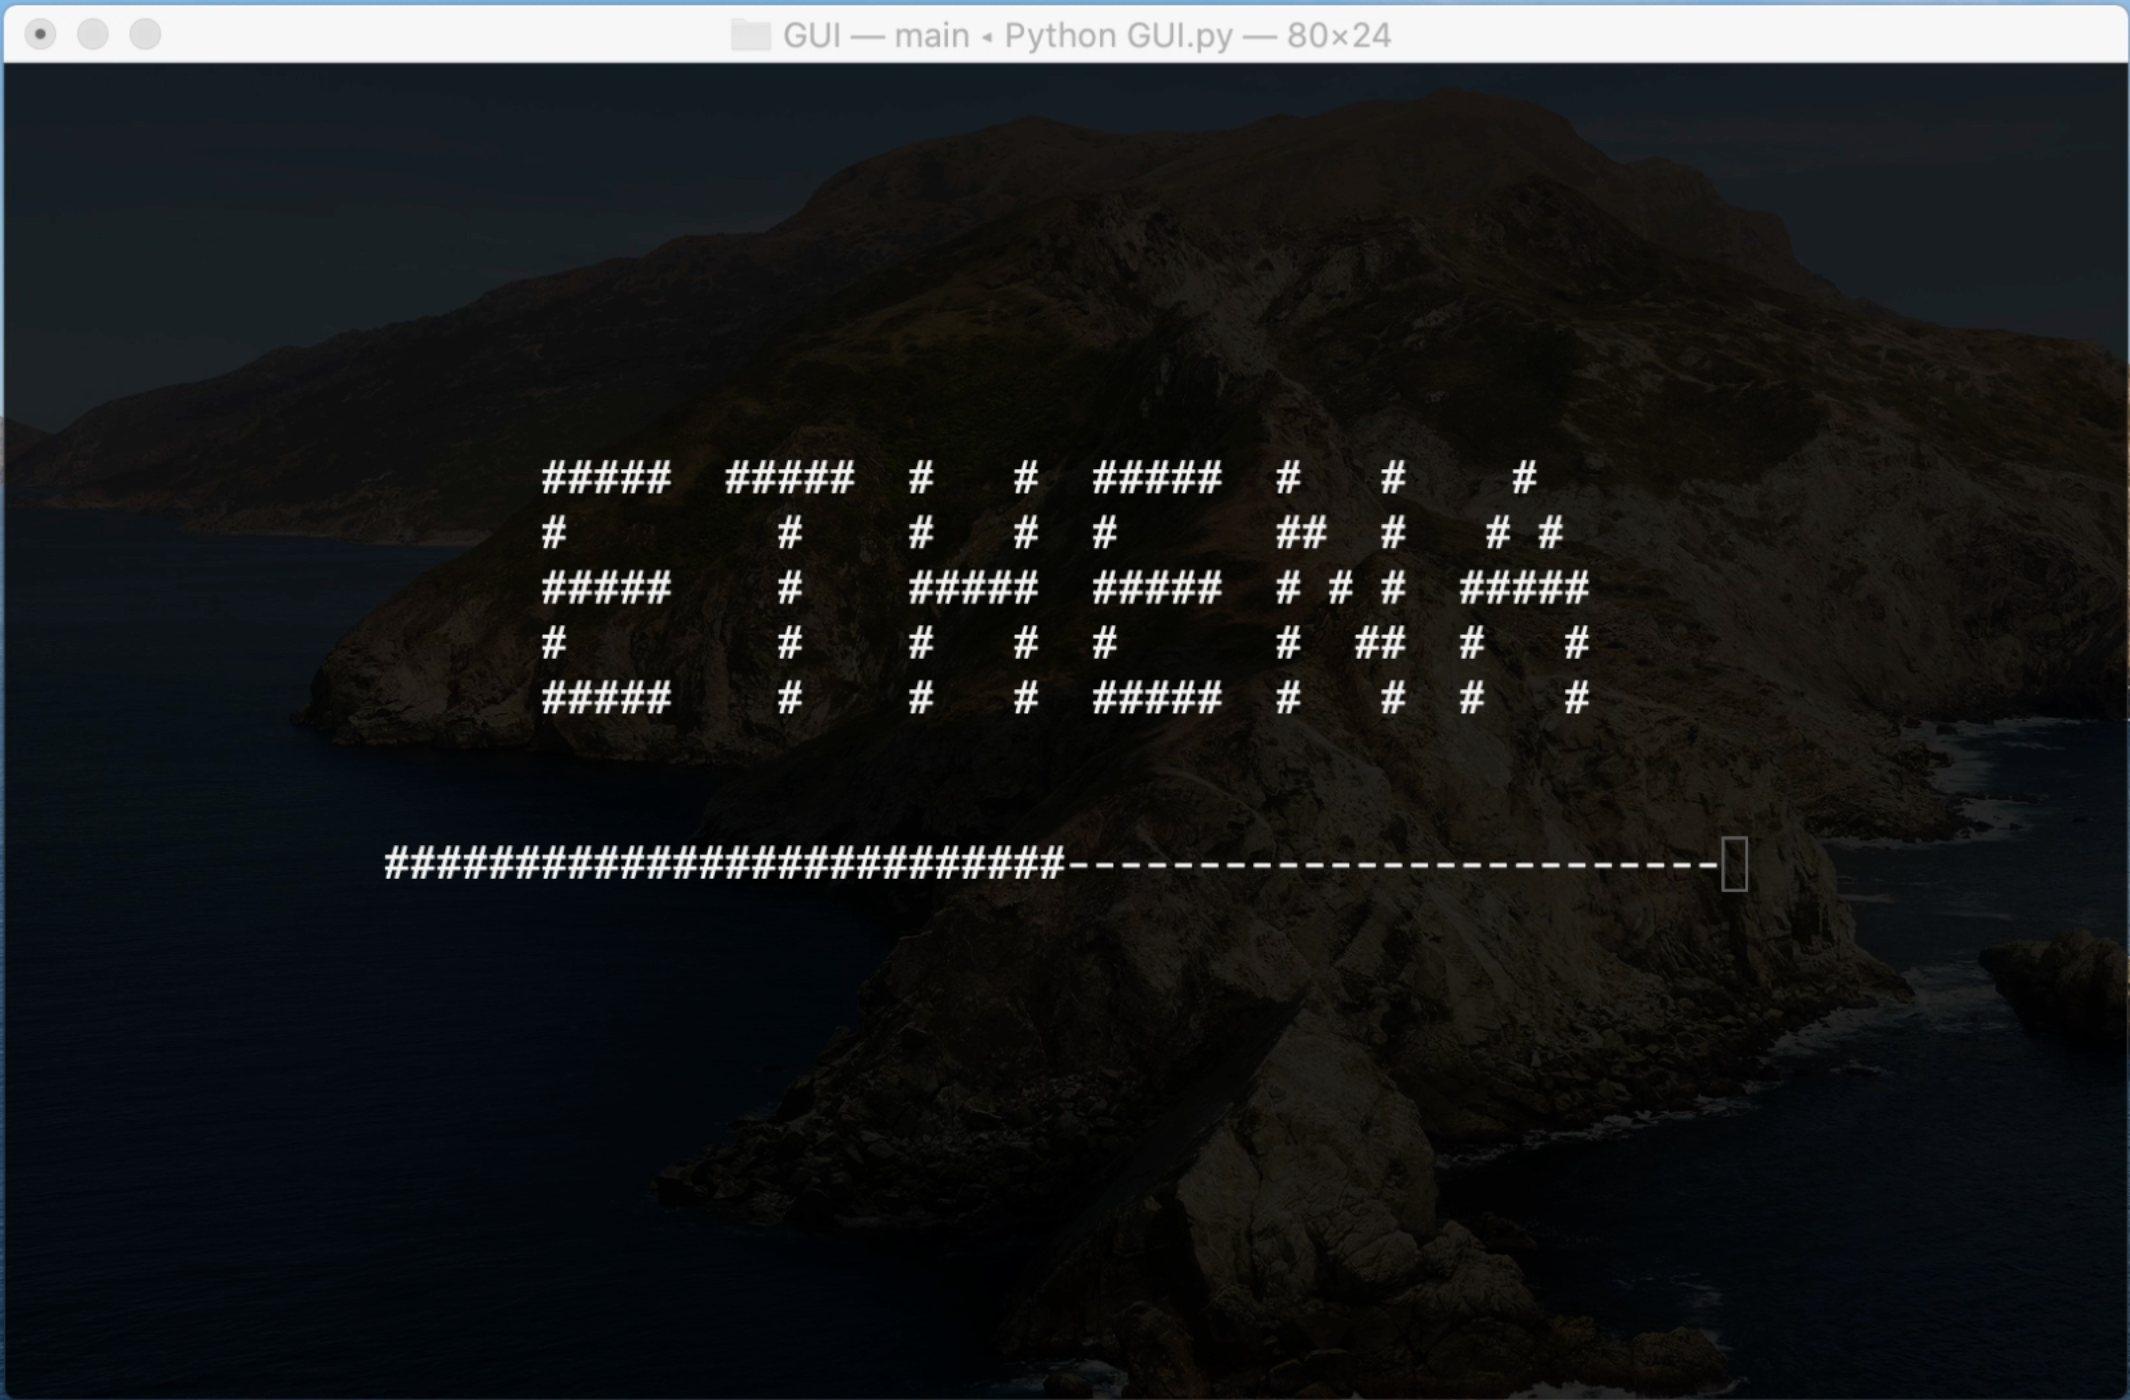
\includegraphics[width =\textwidth]{LoadingScreen.png}
        \centering
        Figure 2: ETHena Loading page
        \vspace{0.25cm}
    \end{minipage}
    
    \begin{minipage}[b]{1\linewidth}
        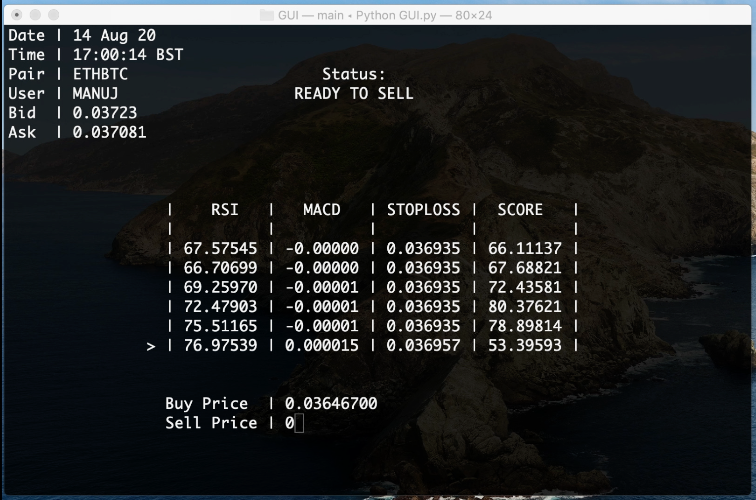
\includegraphics[width =\textwidth]{TUI.png}
        \centering
        Figure 3: ETHena TUI
    \end{minipage}

    \section{Tools and Technologies}
    The primary programming language for this project was Go. Python was used initially to assist in data analysis and graphing when measuring the performance of each strategy. It was also used to create a front end GUI for a more user-friendly experience.

    \section{Conclusion}
    We have thoroughly enjoyed working on this project. Not only has it improved our programming skills significantly, it has provided us with greater knowledge of technical analysis within the trading sphere. We have each learnt a lot and are particularly proud of the effort that we've put in to produce a program this complex.


    \section{Contributors}
    This project was implemented by five 1\textsuperscript{st} year students at Imperial College London. Below are the backgrounds of our team contributors:
    \\
    \subsection{Sanchit Ajmera}
    \vspace{-0.375cm}\textbf{\footnotesize{Joint Mathematics \& Computing}} \\ \\
    Having a strong background in mathematics and an awareness of economics, allowed me to contribute to the project by designing a scalable structure with Manuj. This set the foundation for the rest of the project and from this, I implemented a model to backtest various trading strategies on historical data. Later on, I aided in the production of additional features including an email notification system, daily update reports and the ETHena TUI.

    \subsection{Luqman Liaquat}
    \vspace{-0.375cm}\textbf{\footnotesize{Computing}} \\ \\
    With a keen interest in computing and experience in Linux, I set up and managed the AWS server instances for the live deployment of ETHena across our accounts. I also worked on anti-loss features for the data collection used within our backtesting facilities to ensure our files remained consistent. Additionally, I assisted Shivam in combining the different trading strategies intuitively. This project has sharpened my skills with the Go programming language and has significantly improved my understanding of technical analysis for trading.

    \subsection{Manuj Mishra}
    \vspace{-0.375cm}\textbf{\footnotesize{Joint Mathematics \& Computing}} \\ \\
    My key contribution in this project were to create the RSI-only bot on which ETHena was based. After working with Sanchit to create the foundation of the codebase, I set up the utilities which allowed ETHena to trade live on the Luno market. As a student of both Mathematics and Computer Science, I was keen to involve myself in every facet of this competition - from the market analysis techniques to the roots of the codebase. I've learnt so much throughout this process and I'm very grateful for the opportunity.

    \subsection{Shivam Patel}
    \vspace{-0.375cm}\textbf{\footnotesize{Mathematics}} \\ \\
    I have years of experience trading in stocks and a strong interest in coding. This hackathon was a great opportunity for me to bring these two interests together. My contribution to this project was providing the trading knowledge to help my team members build the bots early on in the project. As my confidence with Go increased and with Luqman's help, I also then implemented all the strategies into a single bot - ETHena - using a weighted system for each strategy.
    \vspace{4cm}
    \subsection{Devam Savjani}
    \vspace{-0.375cm}\textbf{\footnotesize{Computing}} \\ \\
    Approaching this project from a computing background, I was very well versed in programming which helped me with the implementation of the GUI. In addition to my technical contributions, I was heavily involved in the research of various strategies including the development of the candlestick analysis strategies which overall greatly developed my trading skills and financial knowledge.
    \section{Acknowledgements}
    We would like to thank Adam Hicks and his team at Luno for their help throughout the competition. We would also like to thank En[code] Club for organising the Spark University Hackathon. Finally, a special thanks to Anthony Beaumont for his continued support and mentorship throughout this project.

    \\We are also grateful for the following people that have enabled us to accomplish this.
    \begin{itemize}
        \item Golang packages
              \begin{enumerate}
                  \item Excelize - xuri
                  \item Tealeg - Geoffrey J. Teale
                  \item gomail.v2 - Alexandre Cesaro
              \end{enumerate}
        \item Python modules
              \begin{enumerate}
                  \item PySimpleGui - PySimpleGui Organisation
                  \item pandas - Wes McKinney
                  \item matplotlib - John D. Hunter, Michael Droettboom et al.
              \end{enumerate}
    \end{itemize}
    To see our demo of ETHena click \href{https://youtu.be/INVkpd85hOY}{here} or visit this link: \href{https://youtu.be/INVkpd85hOY}{https://youtu.be/INVkpd85hOY}.
\end{multicols}
\newpage
\section{Appendix}
\begin{figure}[h!]
\includegraphics[angle=270, scale=0.53]{{Graph.png}}
\centering
\caption{Graph of trading on 16-Aug}
\end{figure}
\end{document}